\documentclass[Royal,times,sageh]{sagej}

\usepackage{moreverb,url,natbib, multirow, tabularx}
\usepackage[colorlinks,bookmarksopen,bookmarksnumbered,citecolor=red,urlcolor=red]{hyperref}



% tightlist command for lists without linebreak
\providecommand{\tightlist}{%
  \setlength{\itemsep}{0pt}\setlength{\parskip}{0pt}}





\begin{document}


\setcitestyle{aysep={,}}

\title{rtoot: Collecting and Analyzing Mastodon Data}

\runninghead{Schoch \& Chan.}

\author{David Schoch*\affilnum{1}, Chung-hong Chan\affilnum{1}}

\affiliation{\affilnum{1}{GESIS Leibniz Institute for the Social
Sciences}}

\corrauth{David Schoch, GESIS Leibniz Institute for the Social
Sciences.}

\email{\href{mailto:david.schoch@gesis.org}{\nolinkurl{david.schoch@gesis.org}}}

\begin{abstract}
An implementation of calls designed to collect and organize Mastodon
data via its Application Program Interfaces (API).
\end{abstract}

\keywords{Mastodon; Social Media; Mobile Platform; API;}

\maketitle

\hypertarget{solution-access-the-mastodon-api}{%
\section{Solution: Access the Mastodon
API}\label{solution-access-the-mastodon-api}}

Mastodon is a free and open source software which allows to run a
self-hosted microblogging service, similar to Twitter. Servers running
Mastodon can interoperate, meaning that their users can communicate
across different instances. Together, all Mastodon instances form a
large decentralized federation of social networking sites. Mastodon was
first released in late 2016 but has not attracted as much attention by
users and researchers compared to centralized social media platforms
such as Twitter. Previous studies on Mastodon
\citep[e.g.~][]{zulli:2020:R, la:2022:NAI} classify it as an
``alternative social media'' platform, in contrast to ``corporate social
media'' platforms such as Twitter. Due to the open source nature,
Mastodon is also famous for being the technology behind far-right social
media platforms Gab and Donald Trump's Truth Social. These far-right
platforms have also captured certain academic attention
\citep[e.g.~][]{zhou:2019:E, zannettou:2018:WG}.

The Twitter takeover by Elon Musk in 2022, however, has changed this
alternative ---if not fringe--- status of the technology and sparked a
huge wave of new registrations for instances running Mastodon
\citep{huang_2022}. Mastodon will become increasingly more relevant for
communication scholars who study online behaviour and phenomena. It is
important to note that Mastodon also is a mobile platform. Official
mobile apps for the platform are recently released, although third-party
mobile apps such as Tusky (Android) and Amaroq (iOS) have long been
available.

Data collection from instances running Mastodon can be facilitated
through the official Mastodon API \citep{mastodonapi} \footnote{Due to
  the decentralized nature of Mastodon, each instance has its own terms
  of service (ToS). Please check those terms to see whether this kind of
  cross-instance data collection is allowed. For instance, despite
  ``scholar.social'' allows API access, its ToS explicitly ban
  unapproved academic research. Also, you are not authorized to transfer
  these data to a third party, e.g.~Google APIs. The research ethics is
  beyond the scope of this software presentation. Please consult
  \citet{zimmer2017internet} for general advice. Consult your ethics
  committees for specific.}. The R package \texttt{rtoot}\footnote{Before
  mid November 2022 (see
  \url{https://github.com/mastodon/mastodon/pull/18583}), a post on
  Mastodon was called a ``toot'', similar to a ``tweet'' on twitter. The
  R package to interact wit the Twitter API is called \texttt{rtweet}
  \citep{rtweet-package}, hence we chose the name \texttt{rtoot}.}
provides functions to authenticate for and interact with this API.

\hypertarget{functionality}{%
\section{Functionality}\label{functionality}}

Many endpoints of the Mastodon API do not require authentication and
calls can be made anonymously. However, instances can decide to require
authentication for some endpoints and user action endpoints, such as
sending a post, require an access token. Setting up a token only needs
to be done once and the function \texttt{auth\_setup()} guides users to
obtain such a token from a particular instance.

Most other functions in \texttt{rtoot} are organized into four groups:
\texttt{get\_instance\_*()} functions for collecting data about an
instance; \texttt{get\_account\_*()} functions for collecting data about
a user account; \texttt{get\_timeline\_*()} functions for collecting
timelines (a series of statuses); and \texttt{stream\_timeline\_*()}
functions for accessing the streaming API. Some exceptions are
\texttt{search\_accounts()} and \texttt{post\_toot()}.

For instance, the following obtains a user access token from the
``emacs.ch'' instance. One can also obtain a public access token, which
can only access public information.

\begin{verbatim}
library(rtoot)
auth_setup(instance = "emacs.ch", type = "user")
\end{verbatim}

The following obtains information about the peers of the instance (other
instances that this particular instance is aware of).

\begin{verbatim}
get_instance_peers(instance = "emacs.ch")
\end{verbatim}

The activity of an instance can be obtained via

\begin{verbatim}
get_instance_activity(instance = "emacs.ch")
\end{verbatim}

All \texttt{get\_account\_*()} functions require a user id instead of
the user name as input. The only way to obtain the user id is to search
for the user name. We have obtained the informed consent from the
account owner of ``chainsawriot'' to collect data from his account.

\begin{verbatim}
search_accounts(query = "chainsawriot")
\end{verbatim}

The following obtains the content published by that account.

\begin{verbatim}
get_account_statuses(id = "109337011845249544",
                     instance = "emacs.ch")
\end{verbatim}

The tibble returned from \texttt{get\_account\_statuses} and any
\texttt{get\_timeline\_*} and \texttt{stream\_timeline\_*} function,
contains a list-column for the application used to post the status. To
extract the name of the application, the following function can be used.

\begin{verbatim}
extract_application <- function(application) {
  if (length(application) == 0) {
    return(NA)
  } else {
    return(application$name)
  }
}
\end{verbatim}

This auxiliary functions allows to filter out statuses that were posted
via a mobile device or directly compare mobile with web-based posts. For
example, one can visualize the length of toots from a mobile device
(iOS) and the web interface (Figure 1).

\begin{verbatim}
library(tidyverse)
x <- get_account_statuses(id = "109337011845249544",
                         instance = "emacs.ch", limit = 30)
x %>% mutate(interface = map_chr(application,
                                 extract_application), 
             length = nchar(content)) %>%
    filter(!is.na(interface)) %>%
    ggplot(aes(x = interface, y = length)) + 
    geom_dotplot(binaxis = "y", stackdir = "center",
                 dotsize = 0.5)
\end{verbatim}

\begin{figure}
\centering
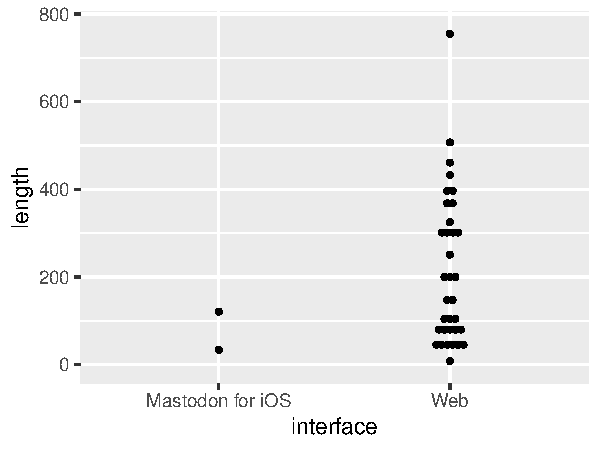
\includegraphics{fig1.pdf}
\caption{Length of toots from different interfaces}
\end{figure}

More information can be found in the github wiki
(\url{https://github.com/schochastics/rtoot/wiki/application}).

\hypertarget{availability-of-the-software-and-tutorials}{%
\section{Availability of the software and
tutorials}\label{availability-of-the-software-and-tutorials}}

\texttt{rtoot} is available on CRAN
(\url{https://cran.r-project.org/web/packages/rtoot/index.html}) and
from the official Github repository
(\url{https://github.com/schochastics/rtoot}). The package contains
tutorials on authentication, streaming, and a general introduction as
vignettes. Additional tips on using the package are available from the
official wiki (\url{https://github.com/schochastics/rtoot/wiki}) and the
online documentation (\url{https://schochastics.github.io/rtoot/}).

\bibliographystyle{sageh}
\bibliography{bibfile}


\end{document}
